\section{Introduction} \label{intro}

Sleep is considered to be ubicuitous and necessary in so far as it was observed in most animal models.

In vertebrate, electrophysiological recordings, in particular, \gls{eeg}, but also \gls{emg}
Classically, activity has been classified in several discrete \emph{vigilance states}...

In rodents, three vigilance states are usually defined on the basis of \gls{eeg} and \gls{emg} (fig.~\ref{fig:sleep_description}).
When awake (WAKE), an animal tends to have a high muscular activity which translates as a high amplitude in the \gls{emg} and a relatively low amplitude
\gls{eeg} domitated by oscilations of frequency between six and ten hertz often refered as theta waves.
In contrast, \gls{rem} sleep, also called slow wave sleep is a period of muscular inactivity (low \ref{emg}) dominated by slow oscilations (below 4Hz) of high amplitude named delat waves.



Annotation of EEG is time consuming and subjective

Recent Effeort to make supervids and unsupervided classifiers.

Advantages and disadvantages of supervided methods.

No general implementation is available/used

Goal is to build an algo that is fast accurate and robust.
It may be baias, but it will be consistant.

Recently, DWD/RF appraoch gave promissing results


This study builds on that using two novelty.

Rigourous testing

Optimised feature extraction python package nwas built. it will be a solid based for future implementation

\Gls{rem}
\Gls{rem}

\begin{figure}[h!]

  \centering    
    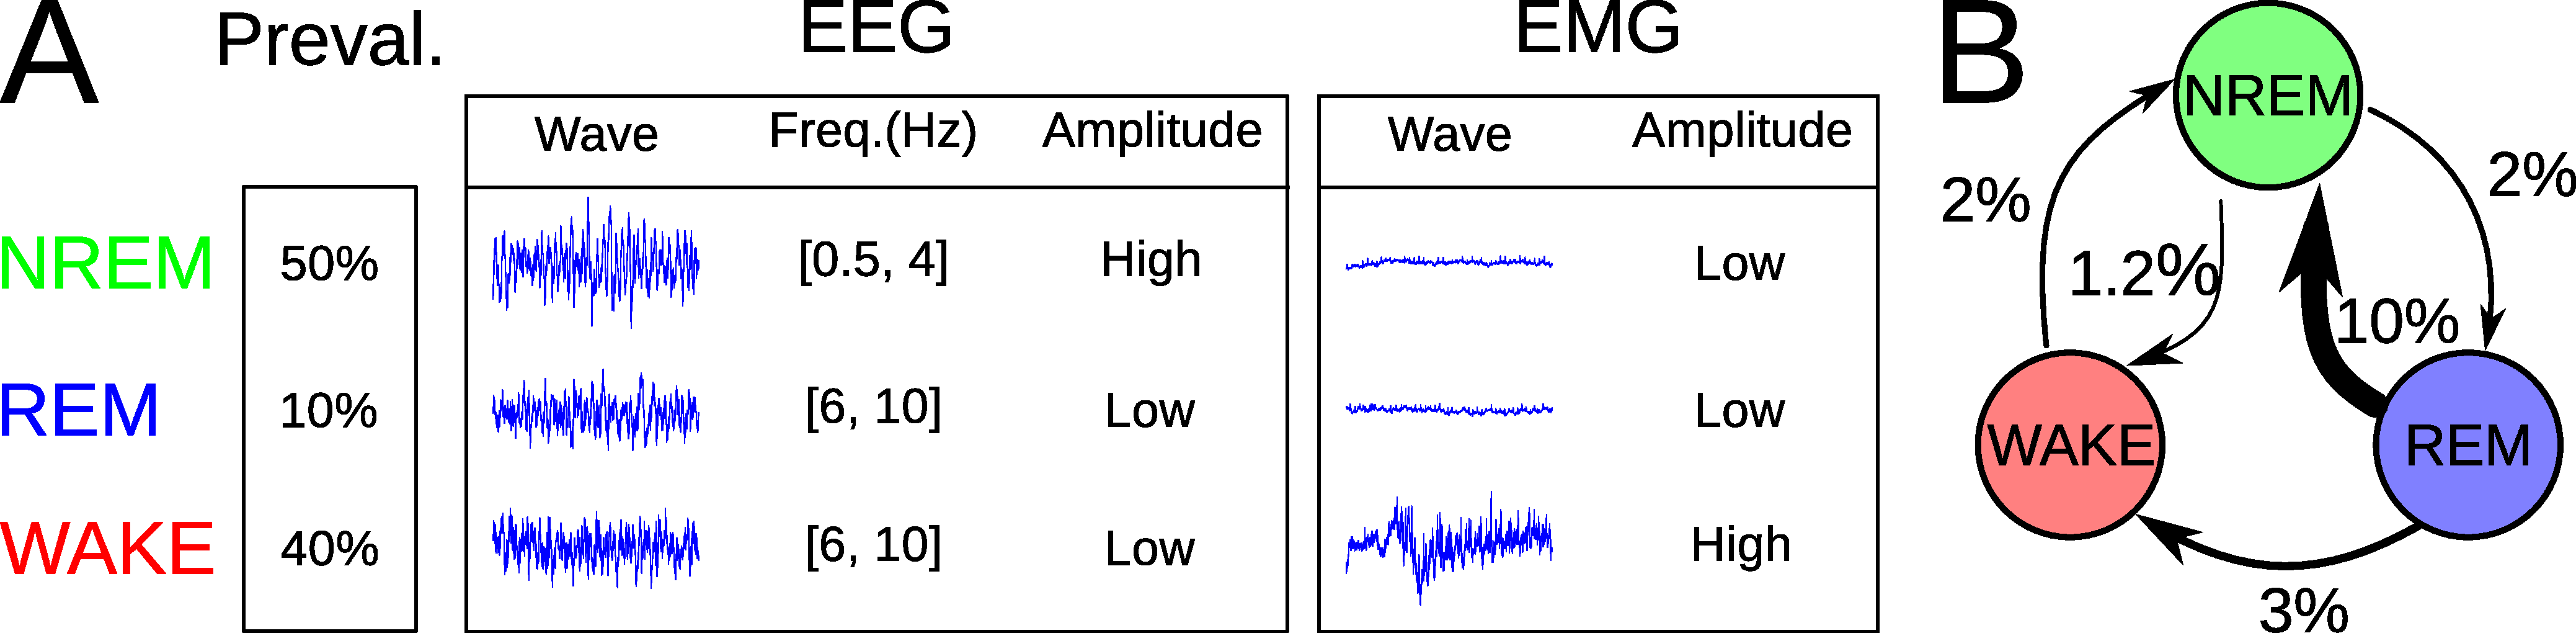
\includegraphics[width=0.95\textwidth]{figures/sleep_description.pdf}
  \caption{\ctit{Structural description of sleep stages.}
  \textbf{A}: Characteristics of the three sleep stages.
  Typically, frequency and amplitude of the \acrfull{eeg}, and amplitude of the \acrfull{emg} are used by experts to infer sleep stage.
  The presented frequency ranges and and pevalences are approximate values for healthy adult animals in normal conditions.
  Each wave shows a representative five second epoch with high signal to noise ratio.
  \textbf{B}: Empirical transition probabilities between consecutive five second epochs. The width of the arrow is proportionnal to the probability of transition.
  Probabilities of remaining in the three state are implied.
  \label{fig:sleep_description}
  }
           
\end{figure}


sgwuaydwui~\ref{fig:sleep_description}

\TODO{an intro is needed}
